\section{Einführung} \label{chap:1}
\subsection{\TeX\ } 
Das Programm worauf \LaTeX\ basiert ist \TeX\ und wurde von Donald E. Knuth im Zeitraum 1977-1986 entwickelt. 
Er war Informatik-Professor an der Stanford University. \TeX\ ist ein Textsatzsystem mit eigener Sprache.
Es liest also Dateien ein und verwandelt diese in z.B. PDFs, welche weiterverwendet und ausgedruckt werden können. Präziser formuliert: Es ist ein Programm, welches aus Quellcode eine Binärdatei generiert, die dann in ein Textdokument umgewandelt werden kann. Man verwendet es zur Erstellung beliebiger Arten von Texten: Dokumente, Bücher, aber auch Dissertationen. \TeX\ wurde in kürzester Zeit als prädestiniertes System für den gesamten wissenschaftlichen Bereich anerkannt. \cite[vgl.][S.1]{Oechsner2015}

\subsubsection{\LaTeX\ }
\paragraph{Namensgebung}\LaTeX\ ist die Abkürzung für \enquote{Lamport \TeX}, benannt nach dem Entwickler Leslie Lamport, wie in Abbildung \ref{fig:leslie} zu sehen. Lamports Entwicklung begann am Anfang der 80er Jahre. \subparagraph{Version} Die aktuelle Version von \LaTeX\ wurde ab 1989 von weiteren Personen, Frank Mittelbach, Chris Rowley und Rainer Schöpf entwickelt. \paragraph{Was ist Latex} \LaTeX\ ist die einfachste und am weitesten verbreitetste Makrosammlung zur Verwendung für \TeX. Ein Makro bezeichnet eine Zusammengefasste Reihenfolge von Anweisungen. Somit wird ermöglicht komplexere Operationen durch einfache Befehle auszuführen. Prinzipiell soll es die Handhabung von \TeX\ vereinfachen und anwenderfreundlicher machen. Die Standardbibilothek von Makros in \LaTeX\ kann vom Benutzer für etliche Formatierungsfälle durch Pakete erweitert werden, die eigene Makros enthalten. \cite[vgl.][S.2]{Oechsner2015}\\
\begin{figure}[H]
    \centering
    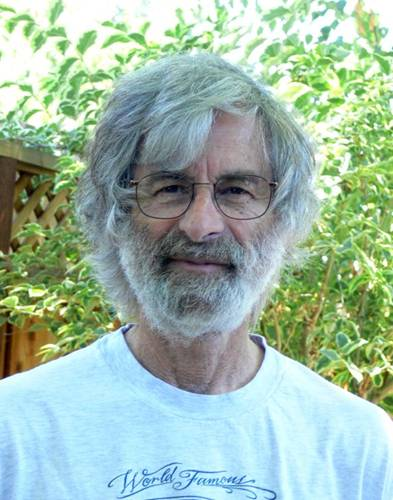
\includegraphics[scale=0.5]{graphics/leslie.jpg}
    \caption[Leslie]{Leslie Lamport}
    \label{fig:leslie}
\end{figure}